\scanpage{66}
% archive sheet number: 65
% The entire draft is cancelled by a long diagonal stroke; two additional nearly vertical cancellation strokes flank the proof.
\deleted{Ceci donne une démonstration plus sympatique et élémentaire de 11.9.6. Quant à 11.9.3. (ii), il varésulter d'un}

\deleted{\uline{Lemme} (ou cor\rlap{l}ollaire à la proposition précédente). Sous les hypothèses de la proposition, ne supposons plus néc que $A'$ soit projectif sur $A$, mais seulement ceci: pour tout quotient intègre $B=A/\underline{p}$ de $A$, posant $B'=B\otimes_A A'$, il existe un $h\quad B-(0)$ tel que $B_h$ soit \mbox{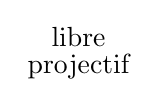
\begin{tikzpicture}[baseline=(base.base)]
\node[inner sep=0] (base) {\deleted{projectif}};
\node[anchor=south,inner sep=0,yshift=.08cm] at (base.north) {\inserted{libre}};
\end{tikzpicture}} sur $A_h$. Alors la conclusion de la proposition reste encore valable.}

\deleted{Soit en effet $\handwritten{\phi}$ une section de $F'$ dont les images par les $u'$ sont nulles, prouvons $\handwritten{\phi}=0$, i.e. $\operatorname{supp}\handwritten{\phi}=\handwritten{\unsure{\varnothing|\phi}}$. Dans le cas contraire, il existerait un point maximal $x'$ dans $\operatorname{supp}\handwritten{\phi}$, correspondant à l'idéal premier $\underline{p}'$ de $A'$. Soit \mbox{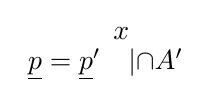
\begin{tikzpicture}[baseline=(base.base)]
\node[inner sep=0] (base) {$\deleted{\underline{p}=\underline{p}'\unsure{\quad|\cap}A'}$};
\path (base.north west) -- coordinate[pos=.60] (ins) (base.north east);
\node[anchor=south,inner sep=0,yshift=.10cm] at (ins) {\inserted{$x$}};
\end{tikzpicture}} son image dans $X$, défini par l'idéal $\underline{p}$ trace de $\underline{p}'$ sur $A$, alors en vertu de l'hypothèse appliquée à $A/\underline{p}$, on voit que, quitte à remplacer $X$ par un voisinage ouvert affine de $x$, on peut supposer que $\rlap{\(B\)}A'/\underline{p}\rlap{\(B\)}A'$ est \mbox{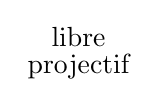
\begin{tikzpicture}[baseline=(base.base)]
\node[inner sep=0] (base) {\deleted{projectif}};
\node[anchor=south,inner sep=0,yshift=.08cm] at (base.north) {\inserted{libre}};
\end{tikzpicture}} sur $A/\underline{p}$. Notons que nous pouvions choisir $x'$ de façon que $x$ soit également maximal dans $g(\operatorname{supp}\handwritten{\phi})$ (commencer par choisir $x$ maximal dans $g(\operatorname{supp}\handwritten{\phi})$, puis $x'$ maximal dans $g^{-1}(x)$), ce qui signifie que localisant en $\underline{p}$, le support de $\handwritten{\phi}_{\underline{p}}$ est contenu dans $\operatorname{Spec}(A'_{\underline{p}}/\underline{p}A'_{\underline{p}})$, donc $\handwritten{\phi}_{\underline{p}}$ est annulé par une puissance de $\underline{p}\ A'_{\underline{p}}$, ou encore que l'on peut trouver $\unsure{\rlap{\(u\)}h|h}\quad A-\underline{p}$ tel que}
